\section{Mô phỏng mạch trên PSpice}
\subsection{Mạch 3.3V regulator}
Đầu tiên, chúng ta sẽ sử dụng đầu vào là nguồn DC 20 V để kiểm thử đầu ra.

\begin{figure}[ht]
    \centering
    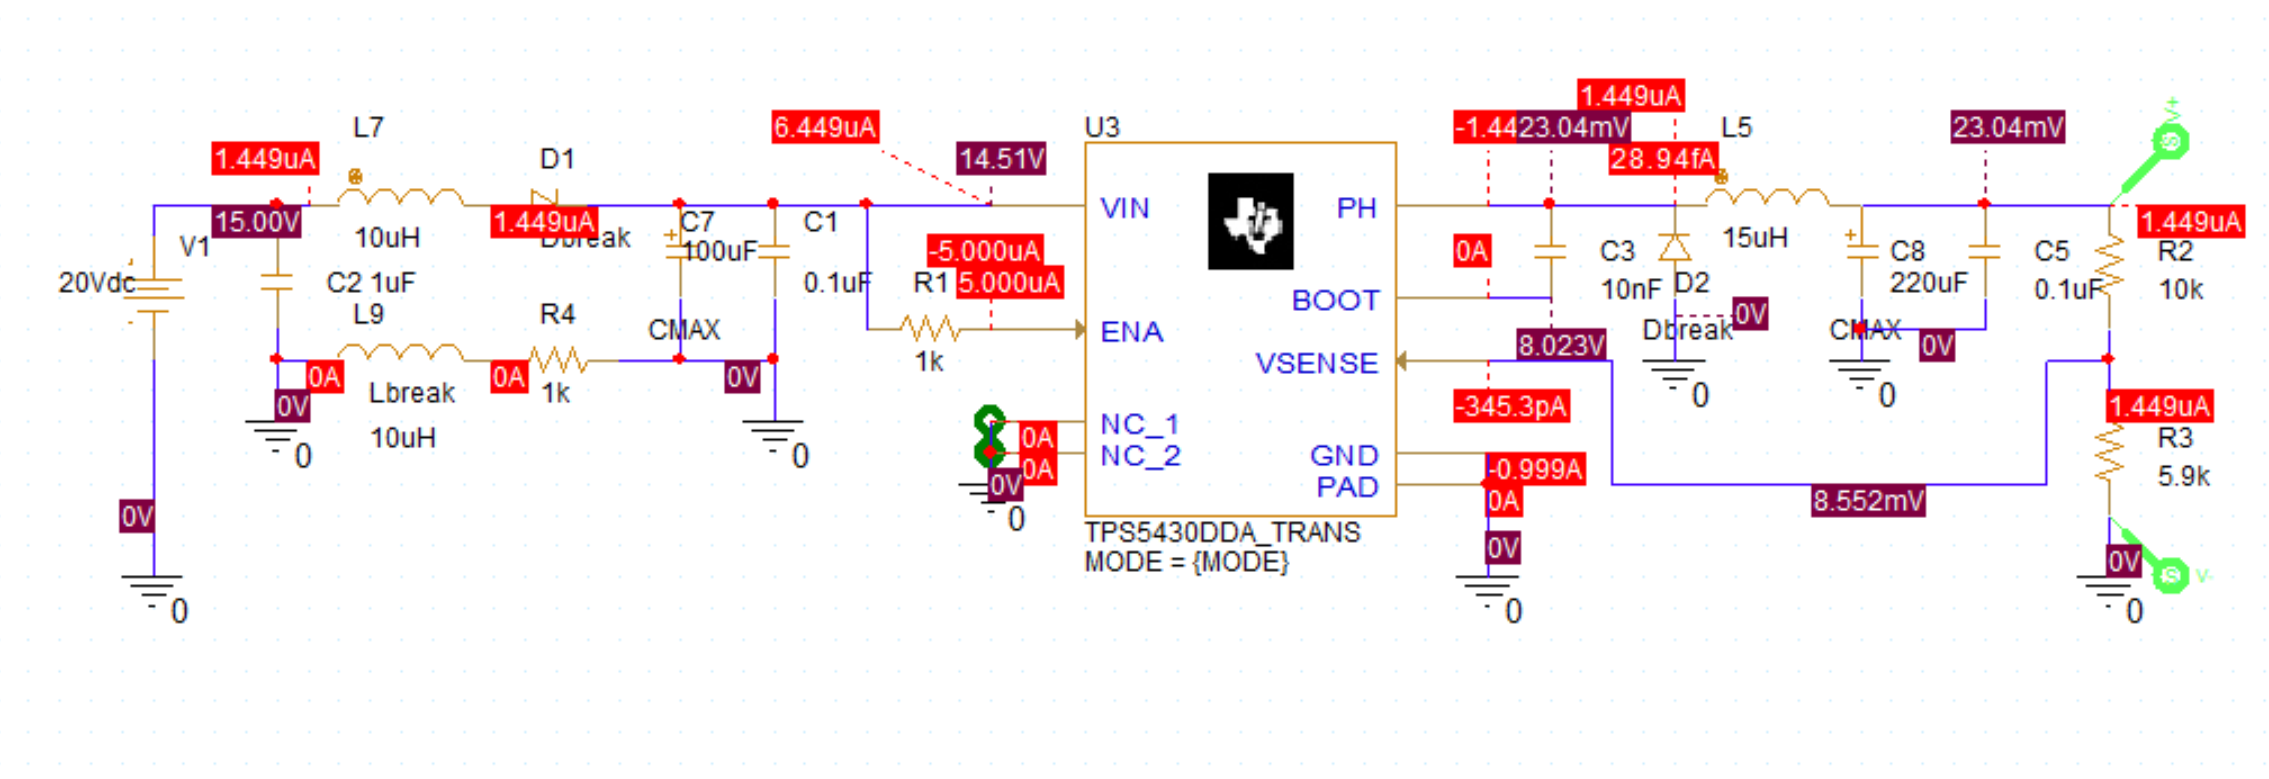
\includegraphics[width=1\textwidth]{graphics/section4/f1.png}
    \caption{Nguồn DC 20 V}
\end{figure}

\textbf{Ảnh mô phỏng}
\begin{figure}[ht]
    \centering
    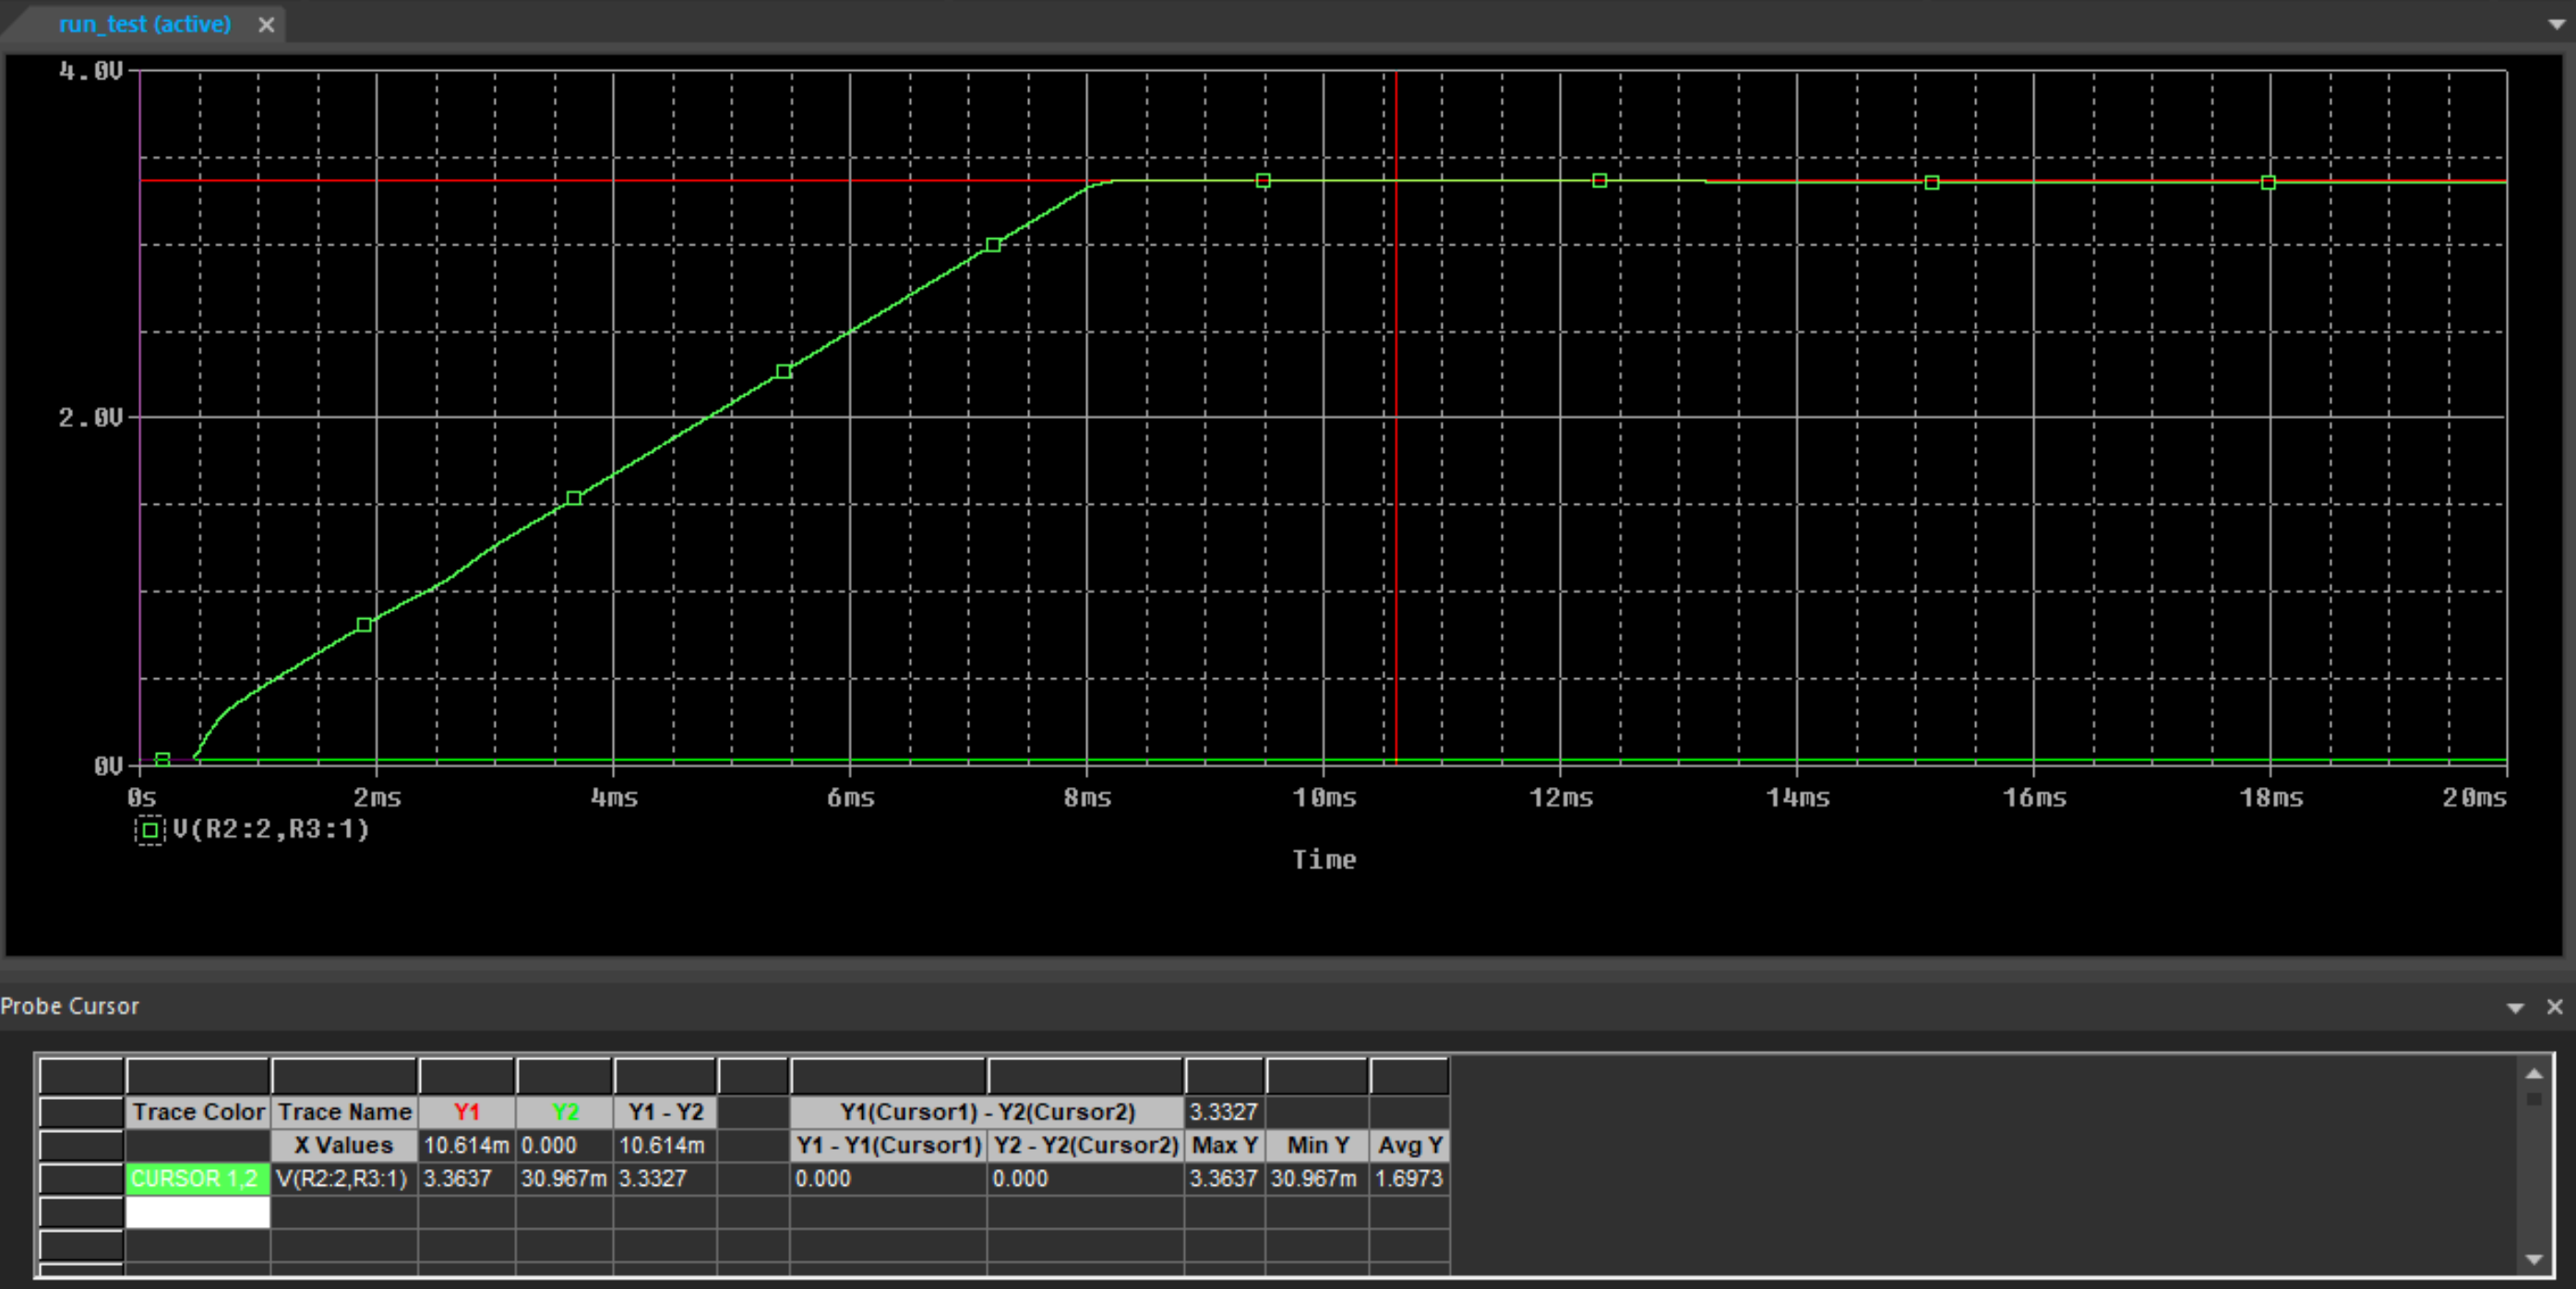
\includegraphics[width=1\textwidth]{graphics/section4/f2.png}
    \caption{Nguồn DC 20 V}
\end{figure}

\textbf{Nhận xét: }Nguồn đầu vào 20 V DC khi qua mạch cho đầu ra ổn định ở mức 3.3V DC. Như vậy, mạch đã hoạt động đúng như yêu cầu.

Tiếp theo ta sẽ cho nguồn đầu vào là tín hiệu AC được dùng như nguồn nhiễu với điện áp gốc (VDC) là 15V và tín hiệu nhiệu (VAC) là 6V.

\begin{figure}[ht]
    \centering
    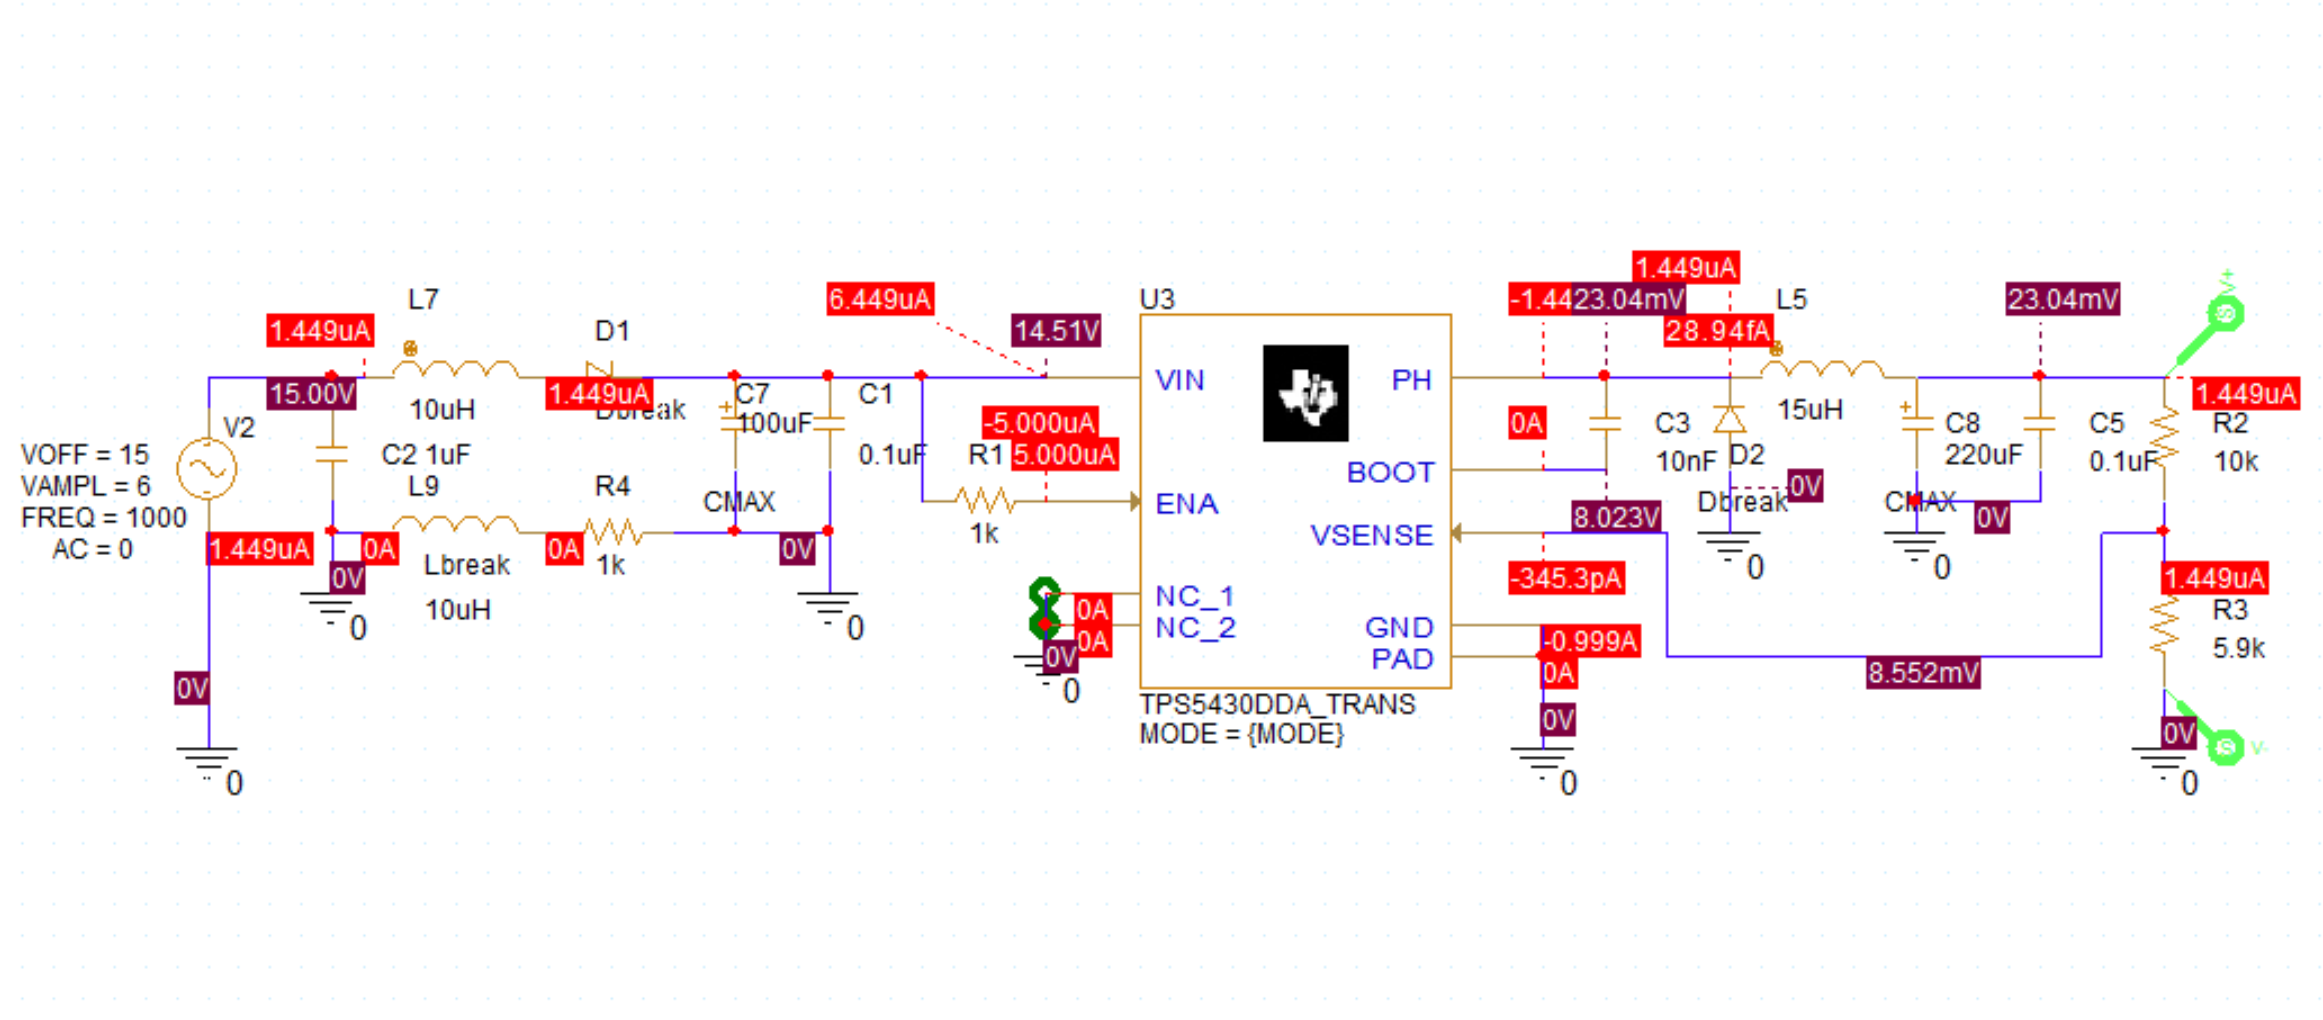
\includegraphics[width=1\textwidth]{graphics/section4/f3.png}
    \caption{Nguồn nhiễu}
\end{figure}

\textbf{Ảnh mô phỏng}
\begin{figure}[ht]
    \centering
    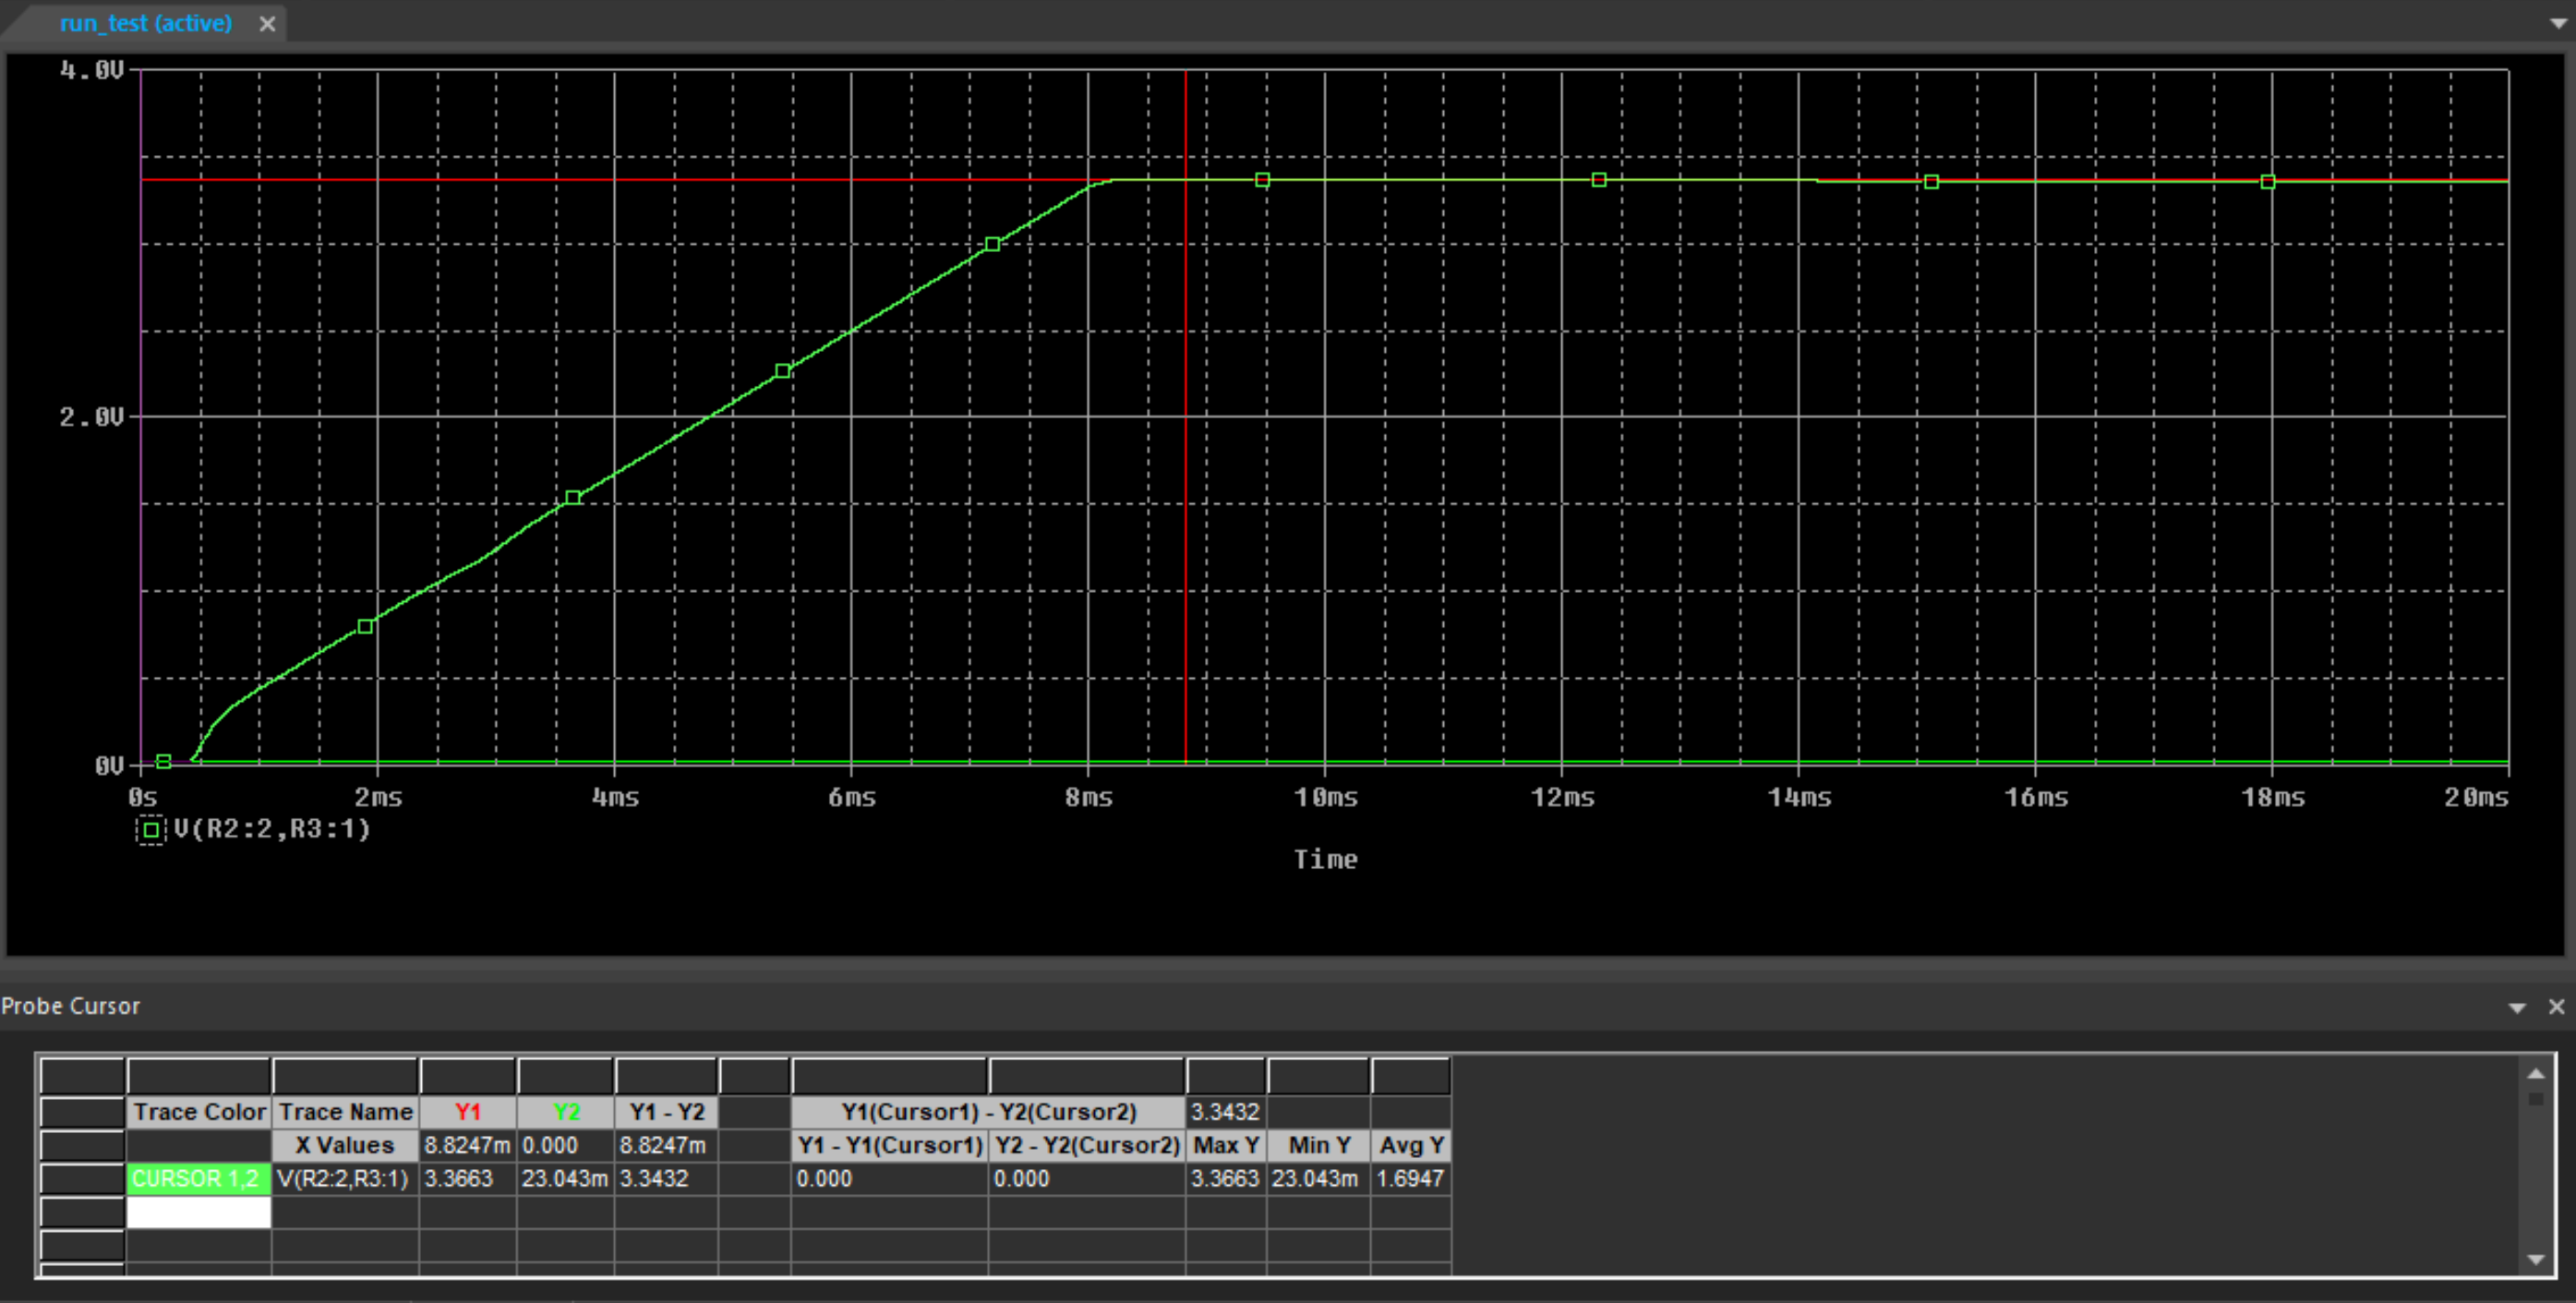
\includegraphics[width=0.95\textwidth]{graphics/section4/f4.png}
    \caption{Nguồn DC 20 V}
\end{figure}

\textbf{Nhận xét: }Mạch đã lọc và giảm áp ổn định ở mức 3.3 V. Như vậy mạch nguồn cần kiểm tra thỏa yêu cầu chức năng.
\pagebreak
\subsection{Current sensor circuit}
\subsection{Interface with high-current LEDs}
